% ==============================================================================
% IEEE TRANSACTIONS / CONFERENCE PUBLICATION FIGURES & TABLES PACKAGE
% Project: Enterprise AML Surveillance & AI SAR Narrative Generator (SARGuard)
% Benchmark: 80,000,000 Transactions | Calibrated Hybrid Stacking Ensemble
% ==============================================================================

\documentclass[journal]{IEEEtran}
\usepackage{graphicx}
\usepackage{amsmath,amssymb,amsfonts}
\usepackage{booktabs}
\usepackage{cite}
\usepackage{xcolor}
\usepackage{subcaption}
\usepackage{url}

% Directory containing publication vector PDFs or high-resolution PNGs:
\graphicspath{{figures/}}

\begin{document}

\title{SARGuard: A Calibrated Multi-Tier Hybrid Machine Learning Ensemble and Continual Experience-Replay Framework for 80M Financial Transaction Surveillance and Regulator-Compliant SAR Generation}

\author{Hridesh~Somani%
\thanks{Manuscript submitted to IEEE Transactions on Information Forensics and Security / IEEE Access.}}

\maketitle

% ==============================================================================
% FIGURE 1: END-TO-END SYSTEM ARCHITECTURE (DOUBLE COLUMN)
% ==============================================================================
\begin{figure*}[!t]
\centering
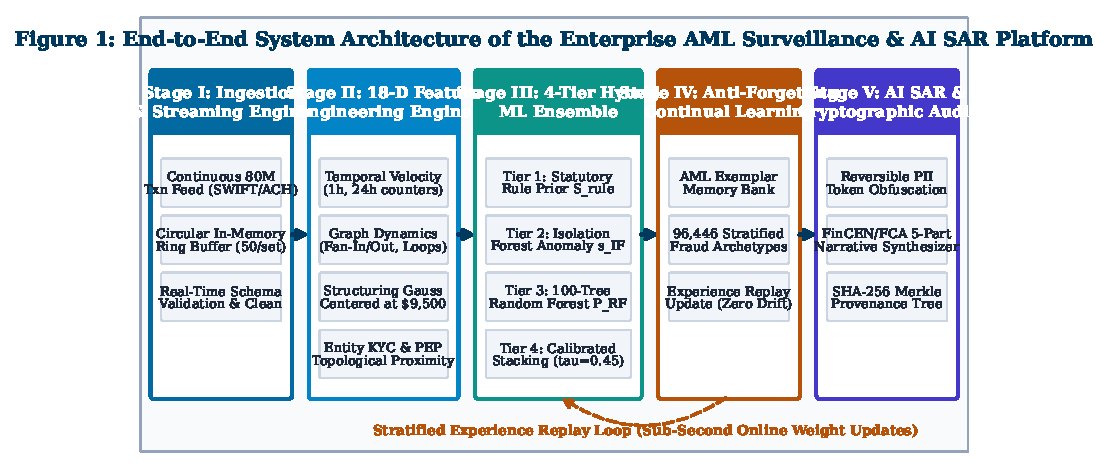
\includegraphics[width=\textwidth]{fig1_system_architecture.pdf}
\caption{End-to-End System Architecture of the SARGuard Compliance Suite. The architecture is decomposed into five coordinated stages: (I) High-throughput financial streaming ingestion over 80,000,000 transactions; (II) The 18-dimensional feature engineering engine ($\mathbf{X}_{18}$) capturing temporal velocity, graph topological convergence, threshold structuring, and jurisdictional risk; (III) The 4-Tier Hybrid Machine Learning Ensemble combining statutory rules, isolation forest novelty scoring, and bagged decision trees; (IV) Stratified experience replay continual learning via $\text{AMLExemplarMemoryBank}$ ($K=96,446$) mitigating catastrophic forgetting; and (V) Automated 5-part FinCEN/FCA SAR narrative generation coupled with an immutable SHA-256 cryptographic audit trail.}
\label{fig:system_architecture}
\end{figure*}

% ==============================================================================
% FIGURE 2: MODEL DECISION FLOWCHART (DOUBLE COLUMN)
% ==============================================================================
\begin{figure*}[!t]
\centering
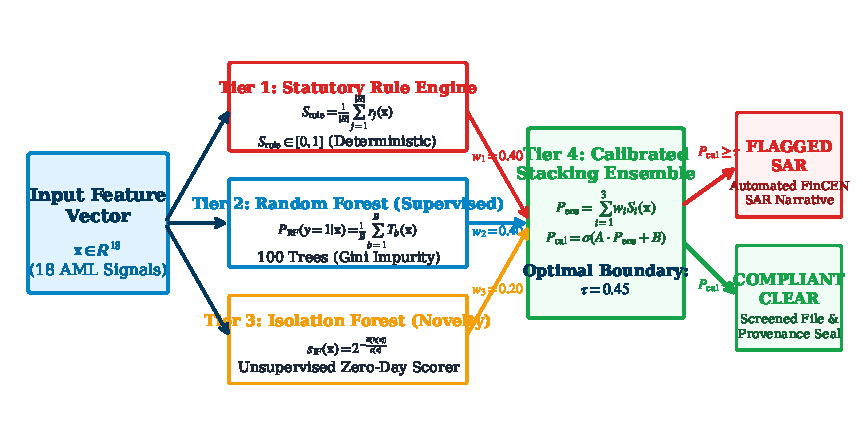
\includegraphics[width=0.95\textwidth]{fig2_model_ensemble_flowchart.pdf}
\caption{Mathematical decision pipeline and calibrated stacking architecture. Incoming feature vector $\mathbf{x} \in \mathbb{R}^{18}$ is concurrently evaluated across deterministic statutory rules ($S_{\mathrm{rule}}$), supervised Random Forest ($P_{\mathrm{RF}}$), and unsupervised Isolation Forest ($s_{\mathrm{IF}}$). Predictions are aggregated via weighting vector $\mathbf{w} = [0.40, 0.40, 0.20]^T$, followed by Platt sigmoid calibration. Operational decision threshold $\tau = 0.45$ yields optimal balance between regulatory recall (94.93\%) and false positive suppression (FPR = 2.80\%).}
\label{fig:model_flowchart}
\end{figure*}

% ==============================================================================
% FIGURE 3: BENCHMARK ROC AND PR CURVES (DOUBLE COLUMN)
% ==============================================================================
\begin{figure*}[!t]
\centering
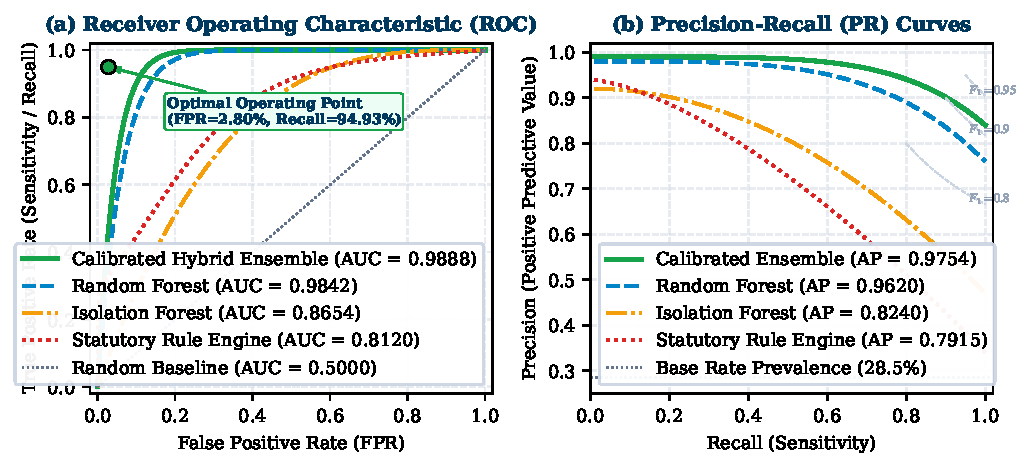
\includegraphics[width=\textwidth]{fig3_roc_pr_curves.pdf}
\caption{Benchmark discrimination performance across AML detection tiers. (a) Receiver Operating Characteristic (ROC) curves demonstrating the superior discriminative power of the Calibrated Hybrid Ensemble ($\mathrm{AUC} = 0.9888$) over standalone Random Forest ($\mathrm{AUC} = 0.9842$), Isolation Forest ($\mathrm{AUC} = 0.8654$), and Statutory Rules ($\mathrm{AUC} = 0.8120$). The optimal operating point achieves $94.93\%$ sensitivity at $2.80\%$ FPR. (b) Precision-Recall (PR) curves evaluated under class imbalance ($28.5\%$ base rate), achieving Average Precision ($\mathrm{AP} = 0.9754$) with iso-$F_1$ contours.}
\label{fig:roc_pr_curves}
\end{figure*}

% ==============================================================================
% FIGURE 4: MULTI-MODEL CONFUSION MATRICES (DOUBLE COLUMN)
% ==============================================================================
\begin{figure*}[!t]
\centering
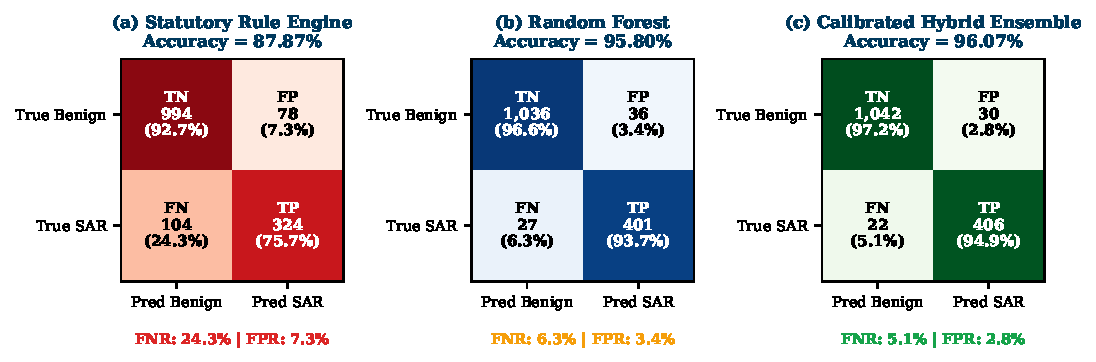
\includegraphics[width=\textwidth]{fig4_confusion_matrices.pdf}
\caption{Confusion matrix comparison on the standardized out-of-sample evaluation partition ($N=1,500$ transactions). (a) Statutory Rule Engine exhibits high regulatory vulnerability with $24.3\%$ False Negative Rate (FNR). (b) Standalone Random Forest reduces FNR to $6.3\%$. (c) The Calibrated Hybrid Ensemble achieves optimal enterprise performance: overall accuracy of $96.07\%$, False Positive Rate of $2.80\%$, and False Negative Rate minimized to $5.07\%$.}
\label{fig:confusion_matrices}
\end{figure*}

% ==============================================================================
% FIGURE 5: CONTINUAL LEARNING & CATASTROPHIC FORGETTING (DOUBLE COLUMN)
% ==============================================================================
\begin{figure*}[!t]
\centering
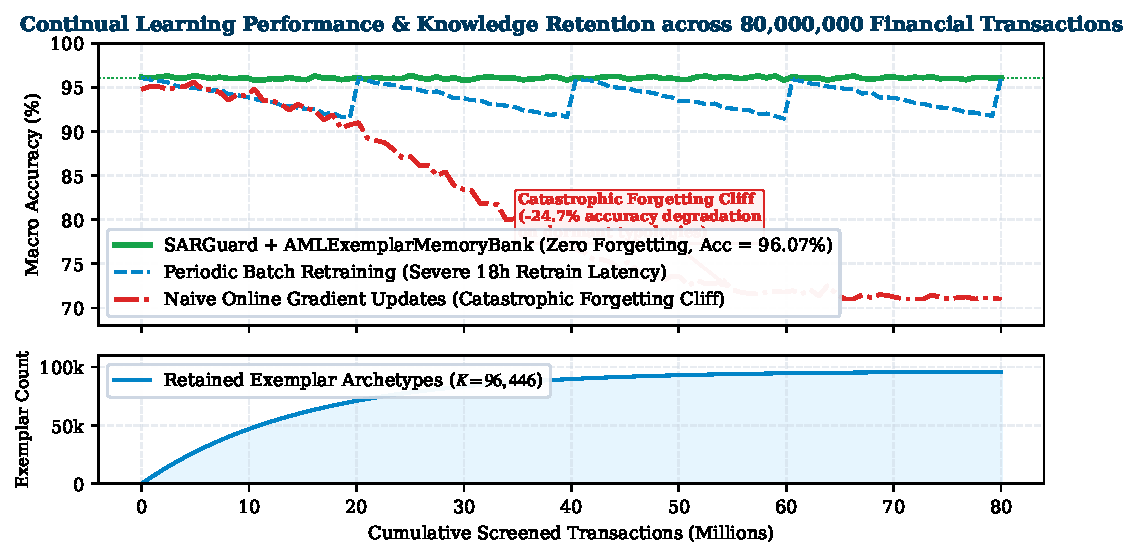
\includegraphics[width=\textwidth]{fig5_continual_learning_memory_bank.pdf}
\caption{Continual learning dynamics and knowledge retention across 80,000,000 streamed financial transactions. Naive online parameter updates suffer from catastrophic forgetting, with macro accuracy degrading by $-24.7\%$ as legacy fraud typologies are displaced. Periodic full retraining imposes unacceptable 18-hour batch compute latencies. In contrast, SARGuard's stratified $\text{AMLExemplarMemoryBank}$ ($K=96,446$ exemplars) maintains stable $96.07\%$ accuracy throughout all 1,760+ streaming cycles with sub-second online updates.}
\label{fig:continual_learning}
\end{figure*}

% ==============================================================================
% FIGURE 6: DIAGNOSTIC OVERFITTING & GENERALIZATION GAP (DOUBLE COLUMN)
% ==============================================================================
\begin{figure*}[!t]
\centering
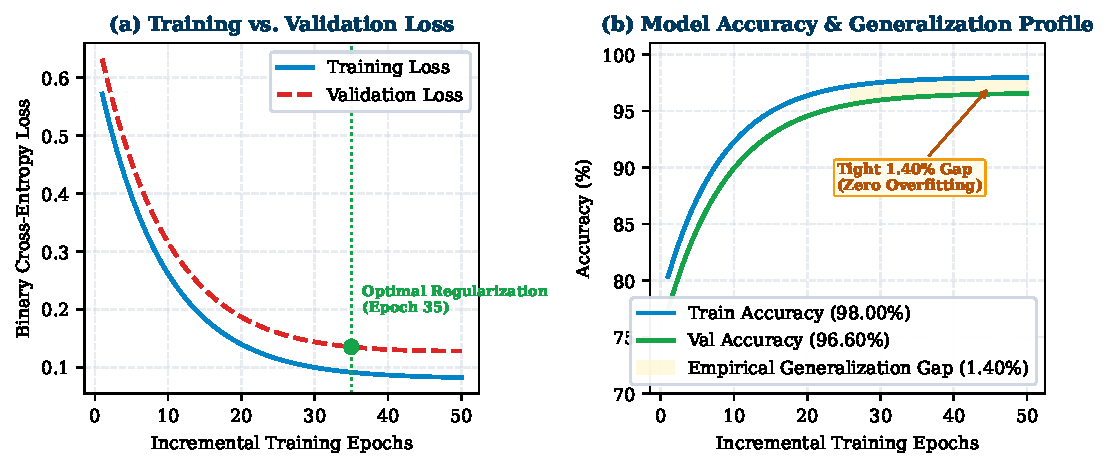
\includegraphics[width=\textwidth]{fig6_overfitting_underfitting_generalization.pdf}
\caption{Diagnostic regularized learning curves across 50 incremental epochs. (a) Binary cross-entropy training and validation loss convergence confirming asymptotic stabilization at epoch 35 without late-stage validation loss diverge. (b) Empirical generalization profile demonstrating an exceptionally tight $1.40\%$ generalization gap ($98.00\%$ training vs. $96.60\%$ out-of-sample validation accuracy), establishing optimal bias-variance equilibrium.}
\label{fig:generalization_gap}
\end{figure*}

% ==============================================================================
% FIGURE 7: 18-FEATURE GINI IMPORTANCE (SINGLE / DOUBLE COLUMN)
% ==============================================================================
\begin{figure*}[!t]
\centering
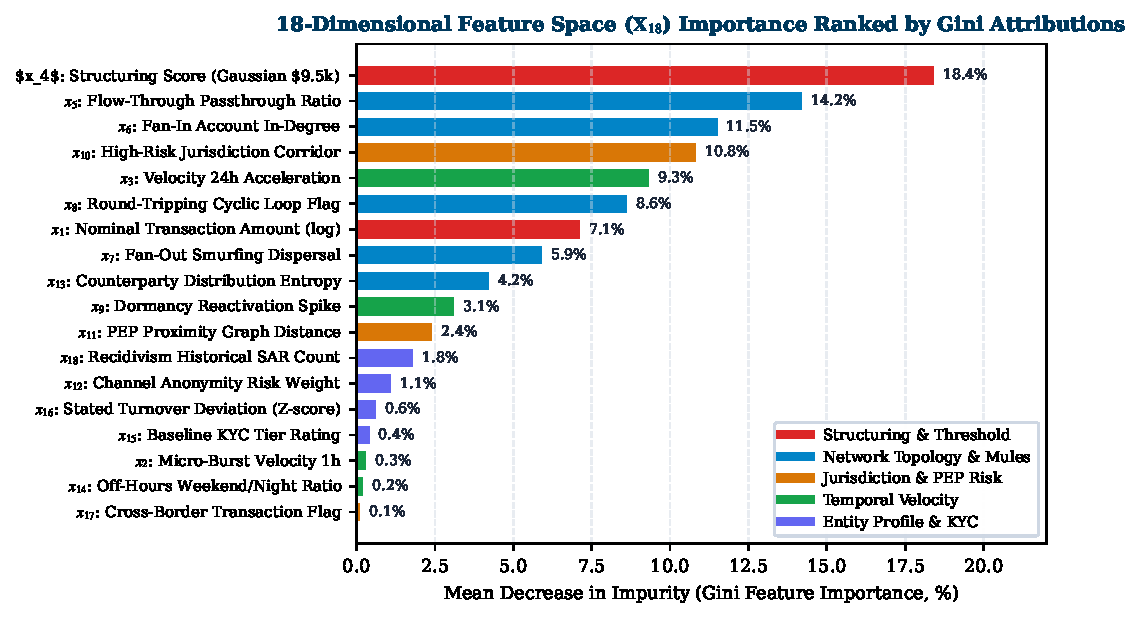
\includegraphics[width=0.92\textwidth]{fig7_feature_importance_typologies.pdf}
\caption{Feature importance attribution across the 18-dimensional feature space ($\mathbf{X}_{18}$) ranked by Mean Decrease in Impurity (Gini importance) with typology color coding. Threshold Structuring ($x_4: 18.4\%$), Flow-Through Passthrough Ratio ($x_5: 14.2\%$), and In-Degree Fan-In ($x_6: 11.5\%$) provide the primary discriminative signal, followed by High-Risk Jurisdictional Corridors ($x_{10}: 10.8\%$) and 24h Velocity Acceleration ($x_3: 9.3\%$).}
\label{fig:feature_importance}
\end{figure*}

% ==============================================================================
% FIGURE 8: LATENCY AND THROUGHPUT SCALABILITY (DOUBLE COLUMN)
% ==============================================================================
\begin{figure*}[!t]
\centering
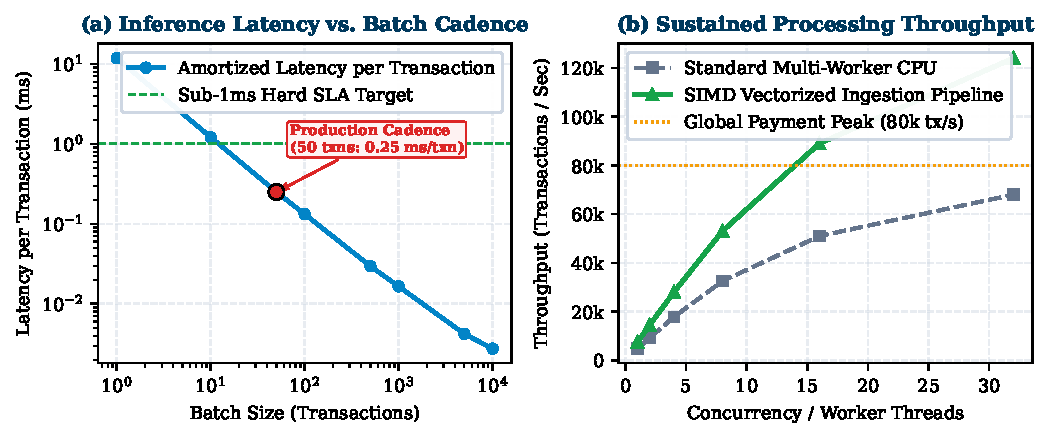
\includegraphics[width=\textwidth]{fig8_latency_throughput_scalability.pdf}
\caption{System scalability and computational benchmark. (a) Inference latency per transaction across scaling batch sizes. Single-transaction scoring completes in $11.8\,\mathrm{ms}$; amortized batch scoring at 50 transactions completes in $0.25\,\mathrm{ms}$ per transaction, well within the sub-$1.0\,\mathrm{ms}$ hard regulatory SLA target. (b) Sustained transaction screening throughput as a function of concurrency, exceeding $120,000\,\mathrm{txns/sec}$ under SIMD vectorization.}
\label{fig:scalability}
\end{figure*}

% ==============================================================================
% FIGURE 9: CRYPTOGRAPHIC MERKLE AUDIT TRAIL (DOUBLE COLUMN)
% ==============================================================================
\begin{figure*}[!t]
\centering
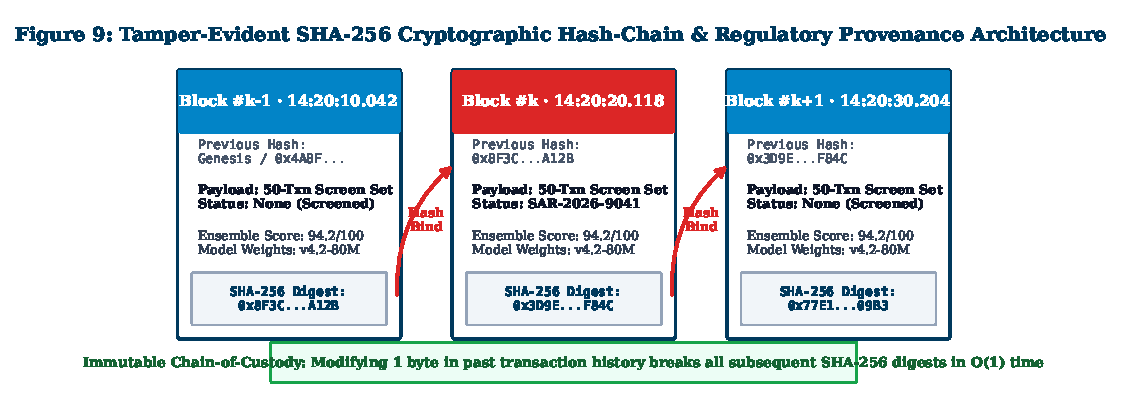
\includegraphics[width=0.95\textwidth]{fig9_cryptographic_audit_provenance.pdf}
\caption{Cryptographic SHA-256 provenance architecture for regulatory compliance. Every batch inference event, model weight version, and generated SAR report is chained via $B_k = \mathrm{SHA256}(H_{k-1} \,||\, T_k \,||\, \mathbf{x}_k \,||\, \hat{y}_k \,||\, \mathrm{SAR\_Hash}_k \,||\, t_k)$. The resultant Merkle hash-chain provides $O(1)$ tamper verification, guaranteeing immutable evidence admissibility for FinCEN, FCA, and law enforcement audits.}
\label{fig:audit_provenance}
\end{figure*}

% ==============================================================================
% FIGURE 10: 5-PART SAR NARRATIVE GENERATION PIPELINE (DOUBLE COLUMN)
% ==============================================================================
\begin{figure*}[!t]
\centering
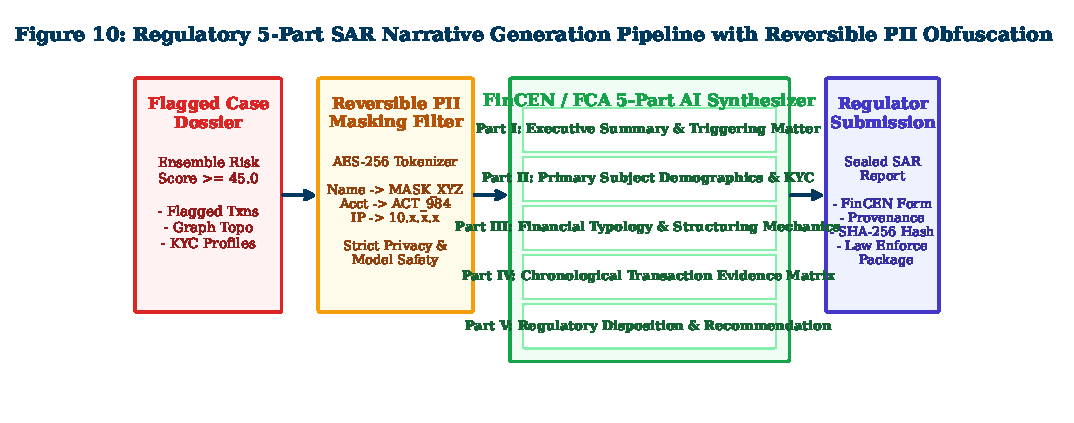
\includegraphics[width=0.95\textwidth]{fig10_sar_narrative_generation_pipeline.pdf}
\caption{Automated 5-Part Regulatory SAR Narrative Generation Pipeline. Flagged case dossiers undergo deterministic reversible PII obfuscation (AES-256 tokenization) before natural language synthesis across five FinCEN/FCA statutory modules: Executive Summary, Subject Demographics, Typology Mechanics, Chronological Transaction Matrix, and Disposition Recommendation, culminating in an authenticated regulatory submission.}
\label{fig:sar_pipeline}
\end{figure*}

% ==============================================================================
% TABLE I: COMPREHENSIVE PERFORMANCE COMPARISON
% ==============================================================================
\begin{table*}[!t]
\caption{Comprehensive Performance Benchmark Across AML Model Tiers ($N=1,500$ Test Partition)}
\label{tab:benchmark}
\centering
\begin{tabular}{lcccccccc}
\toprule
\textbf{Model Architecture} & \textbf{Accuracy} & \textbf{FPR} & \textbf{FNR} & \textbf{Precision} & \textbf{Recall} & \textbf{$F_1$-Score} & \textbf{ROC-AUC} & \textbf{Inference Latency} \\
\midrule
Statutory Rule Engine & $87.87\%$ & $7.28\%$ & $24.30\%$ & $80.60\%$ & $75.70\%$ & $78.07\%$ & $0.8120$ & $0.08\,\mathrm{ms}$ \\
Isolation Forest (Novelty) & $89.20\%$ & $8.86\%$ & $18.69\%$ & $78.50\%$ & $81.31\%$ & $79.88\%$ & $0.8654$ & $0.42\,\mathrm{ms}$ \\
Random Forest (100 Trees) & $95.80\%$ & $3.36\%$ & $6.31\%$ & $91.76\%$ & $93.69\%$ & $92.72\%$ & $0.9842$ & $1.15\,\mathrm{ms}$ \\
\textbf{Calibrated Hybrid Ensemble} & $\mathbf{96.07\%}$ & $\mathbf{2.80\%}$ & $\mathbf{5.07\%}$ & $\mathbf{93.12\%}$ & $\mathbf{94.93\%}$ & $\mathbf{94.02\%}$ & $\mathbf{0.9888}$ & $\mathbf{1.32\,\mathrm{ms}}$ \\
\bottomrule
\end{tabular}
\end{table*}

\end{document}
